\chapter{Effektmoduler}\label{chap:DSP}

\husk{Emil}{ved ikk eom den skulle have et bedre navn}

\section{Reverb effektmodul}\label{sec:reverb}
\husk{Emil}{jeg er ikke helt sikker på opbygningen af denne sektion..}
Reverb, rumklang, er resultatet af lydbølger som bliver reflekteret tilbage af samtlige overflader med forskellige vinkler.\newline
Rumklang er resultatet af lydbølger som bliver reflekteret af samtlige overflader i et rum, derved bygges der en masse reflektioner op hvis amplitude falder mod $0$ som de bliver absorberet af overfladerne i rummet.\newline
Der er to primære metoder for implementeringen af en digital reverb effekt.
Der er convolution (foldnings) reverben og den algoritmiske reverb.
\subsection{Convolution reverb}
Reverberation, rumklang, er en tidsinvariant effekt, hvilket betyder at det ikke har nogen betydning, hvornår en tone bliver spillet, det vil ultimativt resultere i præcis den samme reverberation. \newline
Med tidsinvariante systemer kan de karakteriseres ved deres impulsrespons.
Convolution reverbs virker ved at lave en foldning af rummets impulsrespons og det lydsignal der sættes på indgange n til reverben.\newline
Dette skaber en realistisk rumklangseffekt, fordi impulsen i dette tilfælde vil være en lyd som holder samme energiniveau ved alle frekvenser.
Efter impulsen bliver spillet vil den blive reflekteret rundt i rummet.
Nogle af reflektionerne møder mikrofonen med det samme mens andre bliver ført rundt i rummet og amplituden af signalerne går mod $0$ pga. overfladerne af objekterne i rummet absorbere energien fra dem.\newline
Multiplikering af hver punkt af impulsresponset med amplituden af samplet giver så rummets respons til den sample.
Dette gøres for hver sample af inputtet og giver overlappende responser som så adderes og resulterer i rumklang.
En ulempe ved convolution reverbs er, at der skal mange beregninger til for at få resultatet.
Hvert sample skal individuelt multipliceres med hvert sample af impulsresponset og adderes.
Hvis der haves $N$ samples og impulsresponset er $M$ samples lang skal der udføres $N+M$ multiplikationer og additioner.
F.eks. hvis der haves et impulsrespons på 1 sekund og der samples med $44.1\si{kHz}$, skal der udføres næsten 2 milliarder multiplikationer og additioner i sekundet.
Antallet af multiplikationer og additioner kan dog reduceres drastisk ved at arbejde i frekvensdomænet i stedet for, da foldning i frekvensdomænet er multiplikation.

Fordelen ved convolution reverbs er at ethvert rum i verden kan imiteres, hvis impulsresponset for det valgte rum haves.\newline
Derudover kan man opfinde rum ved at syntetisere et impulsrespons.

\subsection{Algoritmisk reverb}
En algoritmisk reverb virker ved at bruge flere forskellige delays og feedback loops til at opbygge en serie af ekkoer, som dør ud over tid.
Det er sammensætningen af de basale byggeblokke som giver karakteristikken på rummet der emuleres.\newline
Et eksempel på en simpel algoritmist reverb effekt er all-pass filteret.
%insert billede af all-pass filter
Her bliver samplet feeded forward til outputtet så lyden bliver spillet med det samme.
Derudover smides samplet ind i en delay buffer.
Rumklangen skabes så af samples fra delay bufferen, som fungerer som opbygningen af ekkoer og feedback loopet som agerer som absorptionen for at skabe aftagende ekkoer.




\husk{Emil}{koden skulle ikke være her alligevel}
\section{Implementering af reverb}
\section{Ekko effektmodul}
	\subsection{Implementering af ekko effekt}
	
\section{Lowpass filter modul}
Som et effektmodul blev der udviklet et FIR (finite impulse response) filter, hvilket vil sige at impulsresponset af filteret falder til nul efter et vist stykke tid.\newline
Et FIR filters overføringsfunktion er givet ved
\begin{equation}
H(z) = b_0 + b_1z^{-1} + \cdots + b_Kz^{-K}
\end{equation}
Hvori $b_i$ er filterets koefficienter.\cite[p.218]{Tan2013}\newline
Filteret og dets koefficienter bliver ved run-time beregnet efter brugeren inputter cutoff frekvensen. Filteret designes og det koefficienter bliver beregnet via frequency sampling metoden.
\pagebreak
\section{Frequency Sampling}
Frequency sampling metoden virker ved at man lader $h(n)$ for $n = 0, 1, \cdots, N - 1$ approksimere filterets impulsrespons, hvilet for FIR filtre er deres koefficienter, og $H(k)$ for $k = 0, 1, \cdots, N - 1$ er de diskrete Fourier transformationskoefficienter.
\begin{figure}[!ht]
	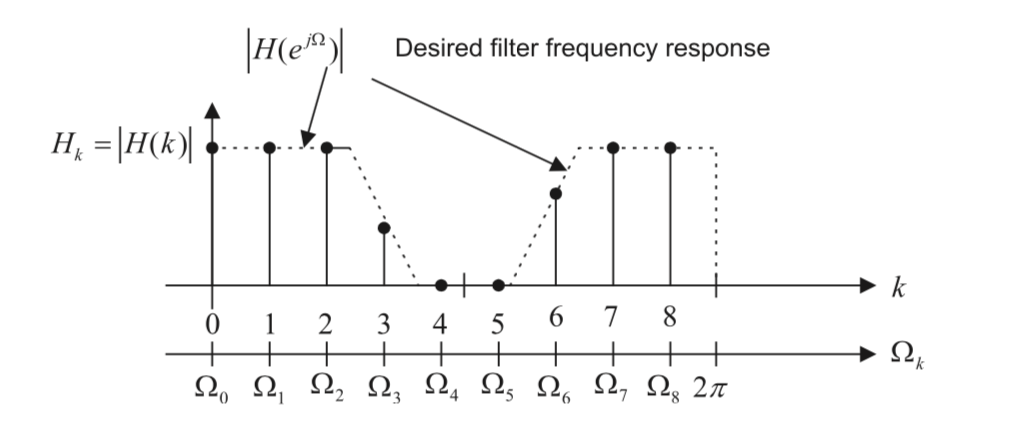
\includegraphics[width=\textwidth]{billeder/frequencysampling.png}
	\caption{Frekvenssampling af amplitudekarakteristik}
	\label{fig:frequencysampling}
\end{figure}
H(k) findes ved at sample den ønskede amplitudekarakteristik i frekvensdomænet ved lige adskilte frekvenser som vist i figur \ref{fig:frequencysampling}.
FIR koefficienterne findes så ved
\begin{equation} \label{eq:fir_koefficienter}
b_n = h(n) = \frac{1}{2M + 1} \left\{H_0 + 2\displaystyle\sum_{k = 1}^{M}\, H_k\cos\left(\frac{2\pi k (n - M)}{2M + 1} \right) \right\} \quad \mathrm{for} \quad n = 0, 1, \cdots, M
\end{equation}
Resten af koefficienterne findes ved $h(n) = h(2M - n) \quad \mathrm{for} n = M + 1, \cdots, 2M$ ved brug af symmetri, når filteret antages at have lineær fase.


\subsection{Implementering af FIR filter}
Det digitale filter blev valgt at blive implementeret som et FIR filter, fordi FIR filtre giver mulighed for at have lineær negativ fase hvilket medfører konstant gruppeløbetid.\newline
Negativ lineær fase medfører konstant gruppeløbetid da gruppeløbetid er givet ved
\[
\tau = \frac{\mathrm{d}\varphi}{\mathrm{d}\omega}
\]
Konstant gruppeløbetid er en fordel at have i audio applikationer da en varierende gruppeløbetid kan komme til at lyde forkert.\newline
Modulet virker ved at det tager en cutoff frekvens som brugerinput og dernæst beregner normerede cutoff frekvens ved
\[ \Omega_c = 2\pi\frac{f_c}{f_s} \]
Hvor $f_c$ er cutoff frekvensen og $f_s$ er samplingsfrekvensen.
Dernæst beregnes en array af amplitudekarakteristikken $H_k$ for de normerede frekvenser fra $0$ til $\pi$ ved 
\[ \Omega_k = \frac{2\pi k}{(2M + 1)} \quad \mathrm{for} \quad k = 0, 1, \cdots, M \]
Når $H_k$ haves beregnes $M$ filterkoefficienter via. \ref{eq:fir_koefficienter} og resten findes ved symmetri.\newline
Filteret virker ved at en buffer fyldes med $x$ samples og dernæst bliver der foretaget en foldning for hver sampel i bufferen med hver filterkoefficient.

